%
% m-kugelfunktionen.tex
%
% (c) 2017 Prof Dr Andreas Müller, Hochschule Rapperswil
%
\chapter{Kugelfunktionen%
\label{skript:chapter:kugelfunktionen}}
\lhead{Kugelfunktionen}
\rhead{}
Im vorangegangenen Kapitel~\ref{skript:chapter:multipol} haben wir
die Multipol-Entwicklung kennengelernt. 
Die wesentliche Erkenntnis dabei war, dass wir eine Funktion immer zerlegen
können in eine Summe von Termen der Form
\[
\frac{p(x,y,z)}{r^k},
\]
wobei $p(x,y,z)$ ein homogenes Polynom in den Koordinaten $x$, $y$ und
$z$ war.
Nehmen wir an,d ass das Polynom homogen vom Grad $l$ ist, dann kann man
auch schreiben
\[
\frac{p(x,y,z)}{r^k}
=
p\biggl(\frac{x}{r},\frac{y}{r},\frac{z}{r}\biggr)\frac1{r^{k-l}}.
\]
Die Brüche $x/r$, $y/r$ und $z/r$ sind konstant entlang eines vom
Nullpunkt ausgehenden Strahls, das Polynom 
\[
p\biggl(\frac{x}{r},\frac{y}{r},\frac{z}{r}\biggr)
\]
ist also eine Funktion, die nur von der Richtung des Strahls
abhängt.
Das Potential lässt sich also schreiben als eine Summe von Termen,
die Produkte sind einer Funktion, die nur von der Richtung abhängig
ist, und einer Funktion, die die Entfernungsabhängigkeit vom Nullpunkt
ausdrückt.

In diesem Abschnitt wollen wir zunächst zeigen, dass man die klassische
Fourier-Theorie genau auf die gleiche Art betrachten kann.
Eine Funktion in der Ebene lässt sich immer beschreiben als eine Summe
von Produkten einer Funktion, die die Richtungsabhängigkeit ausdrückt, und
und einer Funktion, die die Entfernungsabhängigkeit codiert.

Die Wahl einer Basis solcher Funktionen ist jedoch nicht eindeutig.
Wenn wir zusätzlich verlangen, dass die Funktionen im Sinne eines noch
zu definierenden Skalarproduktes orthonormiert sind, dann ist die
Berechnung der entsprechenden Koeffizienten besonders einfach und
führt auf die klassische Fourier-Theorie.

Im letzten Abschnitt wollen wir dann zeigen, dass dasselbe Programm
auch im $\mathbb R^3$ durchführbar ist, und dann auf die Kugelfunktionen
führt.

\section{Approximation mit Polynomen
\label{skript:section:approximation}}
In Kapitel~\ref{skript:chapter:multipol} haben wir gelernt, dass es
sinnvoll sein kann, Funktionen in zwei oder drei Dimensionen zu 
approximieren als Summe von Funktionen, die sich faktorisieren lassen
ein einen Teil, der nur vom Radius $r$ abhängt, und einen Faktor,
der eine Funktion auf einem Kreis oder auf einer Kugeloberfläche
ist, parametrisiert durch den Polarwinkel $\varphi$ im Falle des
Kreises oder der geographischen Breite $\vartheta$ und der geographsichen
Länge $\varphi$ im Falle der Kugel.
Für den Fall des Potentials haben wir in der Form der Multipolentwicklung
eine solche Darstellung gefunden.
Es stellt sich damit aber automatisch die Frage, ob eine solche
Darstellung für beliebige Funktionen überhaupt möglich ist.

\begin{satz}[Weierstrass]
\label{skript:satz:weierstrass}
Sei $X\subset\mathbb R^n$ eine abgeschlossene und beschränkte Teilmenge.
Dann lässt sich jede stetige Funktion $X\to\mathbb R$ beliebige genau durch
Polynom $p(x_1,\dots,x_n)$, $x_i\in\mathbb R$
approximieren.
Speziell gibt es für jede Zahl $\varepsilon>0$ ein Polynom $p(x_1,\dots,x_n)$
derart, dass
\[
|f(x_1,\dots,x_n)- p(x_1,\dots,x_n)|<\varepsilon
\]
für alle $(x_1,\dots,x_n)\in X$.
\end{satz}

Der Satz von Weierstrass ist ein Spezialfall eines wesentlich allgemeineren
Resultates.
Die in Satz~\ref{skript:satz:weierstrass} verwendeten Polynome entstehen
durch algebraische Operationen aus den Funktionen
\[
f_1(x_1,\dots,x_n)=x_1,\qquad
f_2(x_1,\dots,x_n)=x_2,\dots
f_n(x_1,\dots,x_n)=x_n.
\]
Diese Funktionen haben die Eigenschaft, dass es für zwei verschiedene
Punkte im Gebiet $X$ immer eine Funktion gibt, mit der diese Punkte
unterschieden werden können.
Denn da zwei verschiedene Punkte auch mindestens eine verschiedene
Koordinate haben, wird die zugehörige Koordinatenfunktion die beiden
Punkte unterschieden können.
Wir fassen diese Eigenschaft in eine Definition
\begin{definition}
Eine Familie von Funktionen $f_i\colon X\to \mathbb R$ {\em trennt Punkte},
wenn es zu jedem Paar von Punkten $p,q\in X$ eine Funktion $f_j$ gibt derart,
dass $f_j(p)\ne f_j(q)$.
\end{definition}
\index{trennt Punkte}

Wir bezeichnen die Menge der stetigen Funktionen $X\to\mathbb R$
mit $C(X,\mathbb R)$ oder $C(X)$, wenn der Wertebereich klar ist.
In der Menge $C(X)$ der stetigen Funktionen $f\colon X\to\mathbb R$ sind
Addition, Subtraktion, Multiplikation von Funktionen und Multiplikation
von Funktionen mit einer Zahl definiert.
Man sagt, die Menge $C(X)$ sei eine Algebra.
\index{Algebra}
Ausserdem gibt es in $C(X)$ einen Begriff für die Norm einer Funktion,
wir setzen
\begin{equation}
\| f\| = \sup_{x\in X}|f(x)|.
\label{skript:multipol:supremum-norm}
\end{equation}
\index{Supremum-Norm}
Damit erhalten wir auch einen Begriff für den Abstand zweier Funktionen:
\[
\|f-g\| = \sup_{x\in X}|f(x)-g(x)|.
\]
Zwei Funktionen haben Abstand $< \varepsilon$, wenn
\[
|f(x)-g(x)| < \varepsilon
\]
gilt für beliebige $x\in X$.
Mit diese Begriff kann man jetzt auch die Konvergenz von Folgen von
Funktionen in $C(X)$ definieren.

Eine Folge $f_n$ von Funktionen auf $X$ heisst eine Cauchy-Folge, wenn 
für grosse $n$ die Funktionen nicht weit auseinander liegen.
Genauer, wenn es für jedes $\varepsilon>0$ ein $N>0$ gibt so, dass
\[
\|f_n-f_m\| < \varepsilon \qquad\text{für}\; n,m>N
\]
gilt, oder gleichbedeutend damit, wenn
\[
|f_n(x)-f_m(x)|<\varepsilon\qquad\text{für}\; n,m>N
\]
gilt.
Man kann auch zeigen, dass die Menge der Funktionen {\em vollständig} ist,
dass also jede Cauchy-Folge von Funktionen in $C(X)$ gegen eine stetige
Funktion konvergiert.

Man sagt, eine Menge $F\subset C(X)$ ist dicht in $C(X)$, wenn die Elemente
von $F$ jedes Element von $C(X)$ beleibig genau approximieren können.
Für jedes $\varepsilon>0$ und jede Funktion $g\in C(X)$ muss es also eine
Funktion $f\in F$ geben, so dass
\[
|f(x)-g(x)|< \varepsilon
\]
gilt für alle $x\in X$.

\begin{satz}[Stone-Weierstrass]
Sei $f_i$ eine Familie von Funktionen auf dem kompakten Gebiet $X$,
die Punkte separiert, dann ist die von den Funktionen $f_i$ erzeugte
Unteralgebra dicht in $C(X)$, oder mit anderen Worten, jede Funktion
in $C(X)$ lässt sich als Polynom in den Funtionen $f_i$ ausdrücken.
\end{satz}

Die Bedingung, dass die Funktionen $f_i$ Punkte trennen müssen, ist
notwendig, wie man wie folgt sehen kann.
Lassen sich die beiden Punkte $p$ und $q$ nicht trennen, dann
ist $f_i(p)=f_i(q)$ für alle $i$.
Also werden auch alle Polynome von Funktionen $f_i$ auf diesen beiden 
Punkten den gleichen Wert annehmen.
Eine stetige Funktion, die in $p$ und $q$ verschiedene Werte annimmt,
kann also grundsätzlich nicht durch Polynome in den Funktionen
$f_i$ approximiert werden.
Da der Satz~\ref{skript:satz:weierstrass} von Stone-Weierstrass
keine weiteren Bedingungen an die Funktionen $f_i$ macht, ist er
in einem gewissen Sinne optimal: die notwendige Bedingung, dass
die Funktionen $f_i$ Punkte trennen müssen, ist auch hinreichend.

\section{Fourier-Theorie}
Betrachten wir eine Funktion $f(x,y)$ in der Ebenen $(x,y)\in\mathbb R^2$.
Aus Kapitel~\ref{skript:chapter:multipol} wissen wir, dass sich die Funktion
$f(x,y)$ schreiben lässt als Summe von Termen der Form $p(x,y)r^k$, wobei
$p(x,y)$ ein homogenes Polynom ist.

Im Moment interessiert uns nur die Richtungsabhängigkeit, so dass wir
die Funktion $f(x,y)$ auf einen Kreis mit Radius $r$ einschränken können.
Aus Abschnitt~\ref{skript:section:approximation} wissen wir ausserdem,
dass wir nach dem Satz~\ref{skript:satz:weierstrass} von Weierstrass
eine stetige Funktionen auf dem Kreis, einer offensichtlich
abgeschlossenen und beschränkten Menge, durch Polynome belieibig
genau approximieren können.

Die Einschränkung von Kapitel~\ref{skript:chapter:multipol}, dass wir
für den richtungsabhängigen Teil nur homogene Polynome in den Koordinaten
verwenden wollten ist kein Hindernis.
Da wir ohnehin mit einer Summe von Funktionen arbeiten, können wir
die Summe noch weiter zerlegen, so dass in jedem einzelnen Summanden nur ein
homogenes Polynom der Koordinaten verwendet wird.

Ein homogenes Polynom $p(x,y)$ vom Grad $l$ erfüllt
\[
p(x,y) = p\biggl(\frac{x}{r},\frac{y}{r}\biggr) r^l.
\]
In Polarkoordinaten ist
\[
\begin{aligned}
\frac{x}{r}&=\cos\varphi
&&\text{und}&
\frac{y}{r}&=\sin\varphi,
\end{aligned}
\]
so dass wir die Funktion $p(x,y)$ in Polarkoordinaten schreiben
können als
\[
p(x,y)=r^l p(\cos\varphi,\sin\varphi).
\]
Für eine Funktion $f(x,y)$ auf einem Kreis um dem Nullpunkt erwarten wir
daher, dass wir sie in Polarkoordinaten schreiben können also eine
Linearkombination Funktionen der Form
\begin{equation}
\cos^k\varphi \sin^{l-k}\varphi,\qquad 0\le k\le l.
\label{skript:kugelfunktionen:produkte}
\end{equation}
Die Potenzen machen die Ausdrücke etwas kompliziert, doch gibt
es eine Reihe von Identitäten für trigonometrische Funktionen,
die erlauben, solche Produkte auf Summen von Funktionen von 
Vielfachen des Winkels zu reduzieren.
Dazu gehören einerseits die Formeln für die Potenzen:
\begin{align*}
\cos^n\vartheta
&=
\begin{cases}
\displaystyle
\frac{2}{2^n}\sum_{k=0}^{\frac{n-1}2} \binom{n}{k}\cos((n-2k)\vartheta)
&\qquad\text{$n$ ungerade}
\\[10pt]
\displaystyle
\frac{1}{2^n}\binom{n}{\frac{n}2}
+
\frac{2}{2^n}\sum_{k=0}^{\frac{n}2-1}\cos((n-2k)\vartheta)
&\qquad\text{$n$ gerade}
\end{cases}
\\
\sin^n\vartheta
&=
\begin{cases}
\displaystyle
\frac{2}{2^n}\sum_{k=0}^{\frac{n-1}2} (-1)^{\frac{n-1}2-k}\binom{n}{k}\sin((n-2k)\vartheta)
&\qquad\text{$n$ ungerade}
\\[10pt]
\displaystyle
\frac{1}{2^n}\binom{n}{\frac{n}2}
+
\frac{2}{2^n}\sum_{k=0}^{\frac{n}2-1}(-1)^{\frac{n}2-k}\binom{n}{k}\cos((n-2k)\vartheta)
&\qquad\text{$n$ gerade}
\end{cases}
\end{align*}
Ersetzt man die Potenzen in~\eqref{skript:kugelfunktionen:produkte}
durch diese Ausdrücke, entstehen immer noch Produkte von jeweils
zwei trigonometrischen Funktionen.
Solche Produkte können aber immer ersetzt werden durch eine
Linearkombination von Funktionen dank der Summen- und Differenzenformeln:
\begin{align*}
\cos\vartheta\cos\varphi
&=
\frac12\bigl(\cos(\vartheta-\varphi)+\cos(\vartheta+\varphi)\bigr)
\\
\sin\vartheta\sin\varphi
&=
\frac12\bigl(\cos(\vartheta-\varphi)-\cos(\vartheta+\varphi)\bigr)
\\
\sin\vartheta\cos\varphi
&=
\frac12\bigl(\sin(\vartheta-\varphi)+\sin(\vartheta+\varphi)\bigr)
\\
\cos\vartheta\sin\varphi
&=
\frac12\bigl(\sin(\vartheta-\varphi)-\sin(\vartheta+\varphi)\bigr)
\end{align*}
Damit ist gezeigt, dass die Funktion $p(\cos\varphi,\sin\varphi)$
geschrieben werden kann als Linearkombination von trigonometrischen
Funktionen von Vielfachen des Winkels:
\[
p(x,y)=p(\cos\varphi,\sin\varphi)
=
\frac{a_0}2
+
\sum_{k=1}^l \bigl(
a_k\cos k\varphi+b_k\sin k\varphi
\bigr).
\]
Wir vermuten daher, dass sich auch die Funktion $f(x,y)$ als Summe
\begin{equation}
f(x,y)
=
\frac{a_0}2
+
\sum_{k=1}^\infty \bigl(
a_k\cos k\varphi+b_k\sin k\varphi
\bigr)
\label{skript:kugelfunktionen:fourierreihe}
\end{equation}
schreiben lässt.

\subsection{Orthogonalität}
Die Funktionen $\cos k\varphi$ und $\sin k\varphi$ sind offenbar 
wesentlich besser geeignet, eine Funktion von $\varphi$ auszudrücken,
als die Potenzen $\sin^k\varphi$ und $\cos^k\varphi$ und ihre Produkte.
Dies wird noch unterstütz durch die folgende Beobachtung.
Zunächst schreiben wir
\begin{align*}
c_0(\varphi)&=\frac{1}{\sqrt{2}}
\\
c_k(\varphi)&=\cos k\varphi
\\
s_k(\varphi)&=\sin k\varphi
\end{align*}
für die Funktionen, die in der
Reihe~\eqref{skript:kugelfunktionen:fourierreihe}
benötigt werden.
Ausserdem verwenden wir als Skalarprodukt von Funktionen
den Ausdruck
\begin{equation}
\langle f,g\rangle
=
\frac1{\pi}
\int_{-\pi}^{\pi}
f(\varphi)g(\varphi)
\,d\varphi.
\end{equation}
Dann kann man ausrechnen, dass die Funktionen $c_k$ und $s_k$ im
folgenden Sinne orthonormiert sind.
Verschiedene Funktionen haben Skalarprodukt $0$:
\begin{align*}
\langle c_0,c_k\rangle
&=
\frac{1}{\pi}\int_{-\pi}^\pi \frac{1}{\sqrt{2}}\cos k\varphi\,d\varphi=0
\\
\langle c_0,s_k\rangle
&=
\frac{1}{\pi}\int_{-\pi}^\pi \frac{1}{\sqrt{2}}\sin k\varphi\,d\varphi=0
\\
\langle c_k,c_l\rangle
&=
\frac1{\pi}
\int_{-\pi}^{\pi}
\cos k\varphi\cos l\varphi
\,d\varphi
=
\frac1{\pi}
\int_{-\pi}^{\pi}
\cos(k-l)\varphi + \cos(k+l)\varphi
\,d\varphi
=0
\\
\langle s_k,s_l\rangle
&=
\frac1{\pi}
\int_{-\pi}^{\pi}
\sin k\varphi\sin l\varphi
\,d\varphi
=
\frac1{\pi}
\int_{-\pi}^{\pi}
\cos(k-l)\varphi - \cos(k+l)\varphi
\,d\varphi
=0
\\
\langle s_k,c_l\rangle
&=
\frac1{\pi}
\int_{-\pi}^{\pi}
\cos k\varphi\sin l\varphi
\,d\varphi
=
\frac1{\pi}
\int_{-\pi}^{\pi}
\sin(k-l)\varphi - \sin(k+l)\varphi
\,d\varphi
=0
\end{align*}
Identische Funktionen haben Skalarprodukt $1$ mit sich selbst:
\begin{align*}
\langle c_0,c_0\rangle
&=
\frac1{\pi}\int_{-\pi}^{\pi}
\frac1{\sqrt{2}}
\cdot
\frac1{\sqrt{2}}
\,d\varphi = \frac{2\pi}{\pi}\frac12=1
\\
\langle c_k,c_k\rangle
&=
\frac1{\pi}
\int_{-\pi}^{\pi}
\cos^2 k\varphi
\,d\varphi
=
\frac1{\pi}\cdot\pi = 1
\\
\langle s_k,s_k\rangle
&=
\frac1{\pi}
\int_{-\pi}^\pi
\sin^2 k\varphi
\,d\varphi
=\frac1{\pi}\cdot\pi = 1.
\end{align*}
Die Funktionen $c_k$ und $s_k$ verhalten sich also in jeder Beziehung
wie orthonormierte Basisvektoren in einem endlichdimensionalen Vektorraum.
In abgekürzter Form können wir diese Eigenschaften auch als
\begin{equation}
\begin{aligned}
\langle c_k,c_l\rangle
&=
\delta_{kl}
\\
\langle c_k,s_l\rangle
&=0
\\
\langle s_k,s_l\rangle
&=
\delta_{kl}
\end{aligned}
\label{skript:kugelfunktionen:ortho}
\end{equation}
schreiben, wobei wie früher
\[
\delta_{kl}=\begin{cases}
1&\qquad k=l\\
0&\qquad\text{sonst}
\end{cases}
\]
ist.
Die Beziehungen~\eqref{skript:kugelfunktionen:ortho} heissen die
Orthogonalitätsrelationen für die Funktioenn $c_k$ und $s_k$.
\index{Orthogonalitätsrelationen}

\subsection{Bestimmung der Koeffizienten $a_k$ und $b_k$}
Die Orthogonalitätsrelationen~\eqref{skript:kugelfunktionen:ortho} erlauben
uns, die Koeffizienten $a_k$ und $b_k$ in der
Reihenentwicklung~\eqref{skript:kugelfunktionen:fourierreihe}
zu finden.
Dazu nehmen wir an, dass sich die Funktion $f(\varphi)$ als Reihe
in den Funktionen $c_k$ und $s_k$ ausdrücken lässt.
Wir setzen also $f(\varphi)$ in der Form
\begin{align*}
f(\varphi)
&=
a_0 c_0(\varphi)
+
\sum_{k=1}^\infty \bigl(a_kc_k(\varphi) + b_ks_k(\varphi)\bigr)
\end{align*}
an und bestimmen die Skalarprodukte
$\langle c_k,f\rangle$ und
$\langle s_k,f\rangle$ wie folgt
\begin{align*}
\langle c_k,f\rangle
&=
\biggl\langle
c_k,
a_0 c_0+\sum_{l=1}^\infty\bigl(a_l c_l + b_l s_l\bigr)
\biggr\rangle
=
a_0\langle c_k,c_0\rangle
+
\sum_{l=1}^\infty a_l\langle c_k,c_l\rangle
=
a_k
\\
\langle s_k,f\rangle
&=
\biggl\langle
s_k,
a_0c_0+\sum_{l=1}^\infty (a_lc_l+b_ls_l)
\biggr\rangle
=
\sum_{l=1}^\infty b_l\langle s_k,s_l\rangle
=
b_k
\end{align*}
Unter Verwendung der Definition des Skalarprodukts $\langle\;,\;\rangle$
finden wir jetzt die Formeln:
\begin{align*}
a_0
&=
\frac1{\pi}\int_{-\pi}^{\pi} f(\varphi)\frac1{\sqrt{2}}\,d\varphi
\\
a_k
&=
\frac1{\pi}\int_{-\pi}^{\pi} f(\varphi)\cos k\varphi\,d\varphi
\\
b_k
&=
\frac1{\pi}\int_{-\pi}^{\pi} f(\varphi)\sin k\varphi\,d\varphi
\end{align*}
Der erste Term der Reihe wird dann
\begin{align*}
a_0c_0(\varphi)
&=
\frac1{\pi}\int_{-\pi}^{\pi} f(\varphi)\frac1{\sqrt{2}}\,d\varphi
\cdot
\frac1{\sqrt{2}}
=
\frac12
\cdot
\frac1{\pi}\int_{-\pi}^{\pi} f(\varphi) \,d\varphi.
\end{align*}
Es ist daher üblich, den Koeffizienten $a_0$ mit der gleichen
Formel wie die $a_k$ für $k>0$ zu berechnen.
Wir vermuten daher den folgenden Satz
\begin{satz}
Eine $2\pi$-periodische stetige Funktion $f(\varphi)$ kann geschrieben
werden als
\begin{equation}
\frac{a_0}2
+
\sum_{k=1}^\infty\bigl(
a_k\cos k\varphi + b_k\sin k\varphi
\bigr),
\label{skript:kugelfuntionen:satz:reihe}
\end{equation}
wobei die Koeffizienten $a_k$ und $b_k$ mit den Formeln
\begin{equation}
\begin{aligned}
a_k
&=
\frac1{\pi}
\int_{-\pi}^\pi f(\varphi)\cos k\varphi\,d\varphi
&
&\text{für $k\ge 0$}
\\
b_k
&=
\frac1{\pi}
\int_{-\pi}^\pi f(\varphi)\sin k\varphi\,d\varphi
&
&\text{für $k>0$}
\end{aligned}
\label{skript:kugelfuntionen:satz:koeffizienten}
\end{equation}
berechnet werden können.
\end{satz}

Bisher haben wir nur gezeigt, dass eine solche Formel plausibel ist.
Wenn die Funktion $f(\varphi)$ als endliche Reihe der
Form~\eqref{skript:kugelfunktionen:fourierreihe}, dann trifft der
Satz zu, wie obige Rechnung gezeigt hat.
Der Satz~\ref{skript:satz:weierstrass} zeigt uns aber, dass der
Satz für stetige Funktionen richtig sein muss, denn aus den Funktionen
$\cos k\varphi$ ind $\sin k\varphi$ lassen sich ja wie früher gezeigt
die Potenzen
$x^k=\cos^k\varphi$ und $y^k=\sin^k\varphi$ gewinnen.

Für noch allgemeinere Funktionen, zum Beispiel für Funktionen, die
nur quadratintegrierbar sind, für die also das Integral
\[
\frac1{\pi}
\int_{-\pi}^{\pi} |f(\varphi)|^2\,d\varphi
\]
existiert, sind die 
Formeln~\eqref{skript:kugelfuntionen:satz:koeffizienten}
für die Koeffizienten immer noch sinnvoll, aber die Approximation
der Funktion $f(\varphi)$ durch die
Reihe~\eqref{skript:kugelfuntionen:satz:reihe}
im Sinne der Supremum-Norm~\eqref{skript:multipol:supremum-norm}
ist nicht mehr garantiert.
Dies wird in der allgemeinen Theorie der Fourier-Reihen bewiesen.

Auch für Funktionen, die bis auf endlich viele Stellen stetig sind,
lässt sich die Konvergenz ausserhalb der Unstetigkeitsstellen beweisen.

\section{Kugelfunktionen}
Die Betrachtungen zur Fouriertheorie haben uns gezeigt, dass Funktionen
auf einem Kreis, also $2\pi$-periodische Funktionen, durch eine
Fourierreihe dargestellt werden können.
Die Basisfunktionen der Forierreihen haben sich aus den
Funktionen $x/r$ und $y/r$ ergeben, indem wir $x/r=\cos\varphi$
und $y/r=\sin\varphi$ gesehen haben.

Jetzt wollen wir diese Ideen auf die dreidimensionale Situation
übertragen.
Wir interessieren uns also für Funktionen auf einer Kugeloberfläche,
die wir der Einfachheit halber als Einheitskugel annehmen können.
Als Koordinatensystem auf der Kugel verwenden wir Kugelkoordinaten mit
\begin{equation}
\frac1r
\begin{pmatrix}
x\\y\\z
\end{pmatrix}
=
\begin{pmatrix}
\sin\vartheta\cos\varphi\\
\sin\vartheta\sin\varphi\\
\cos\vartheta
\end{pmatrix}.
\end{equation}
Die Abhängigkeit von $\varphi$ kann natürlich wie bei einer Funktion
auf einem Kreis durch die Fourier-Theorie dargestellt werden.
Die Abhängigkeit von $z/r=\cos\vartheta$ muss sich als ein Polynom
in $\cos\vartheta$ ausdrücken lassen.

\subsection{Homogene Polynome}
In der Fourier-Theorie haben wir gesehen, dass sich eine Funktion
auf dem Kreis als Summe homogener Polynome beschreiben lässt.
Grund dafür war der Satz~\ref{skript:satz:weierstrass}, welcher
garantierte, dass man eine Funktion mit Polynomen beliebig genau
approximieren kann.

Für Funktionen auf der Kugel gilt dies natürlich auch, jede stetige
Funktion auf der Oberfläche der Einheitskugel lässt sich als Polynom in
$x$, $y$ und $z$ schrieben.
Andererseits diese Koordinaten durch Potenzen von trigonometrischen
Funktionen von $\vartheta$ und $\varphi$ ausgedrückt werden können.
Diese können wie früher auch durch Funktionen der Vielfachen Winkel
ausgedrückt werden.

Wir möchten aber sogar noch einen Schritt weiter gehen.
Bereits die Funktionen $\cos\varphi$, $\sin\varphi$ und $\cos\vartheta$
separieren Punkte auf der Kugel, aus folgendem Grund.
Zwei Punkte auf der Kugel unterscheiden sich in mindestens einer 
Koordinate.
Unterscheiden sie sich in $\vartheta$, dann unterscheiden sich auch
die zugehörigen Werte von $\cos\vartheta$, da der Kosinus auf dem
Interval $[0,\pi]$ injektiv ist.
Unterscheiden sie sich in $\varphi$, dann beschreibt
$(\cos\varphi,\sin\varphi)$ für die beiden Werte von $\varphi$ verschiedene
Punkte auf einem Einheitskreis, also muss mindestens eine der
Komponenten $\cos\varphi$ oder $\sin\varphi$ verschieden sein.
Nach dem Satz~\ref{skript:satz:stone-weierstrass} muss es also schon
möglich sein, durch Potenzen auch nur von $\cos\vartheta$

Man kann dies auch wie folgt verstehen.
Die Wurzelfunktion auf dem Interval $[0,1]$ kann durch ein Polynom $p(x)$
beliebig genau approximiert werden.
Die Sinusfunktion $\sin\vartheta$ wird daher durch die Funktion
$p(1-\cos^2\vartheta)$ beliebig genau approximiert.
Es ist also nicht nötig, die Funktion $\sin\vartheta$ zur Approximation
von Funktionen auf der Kugeloberfläche explizit heranzuziehen.

Wir schliessen aus dieser Argumentation, dass es möglich sein müsste,
Eine Basis von Funktionen zu finden, die die Form
\[
P(\cos\vartheta) \cos(m\varphi)
\qquad
\text{bzw.}
\qquad
P(\cos\vartheta) \sin(m\varphi)
\]
haben.
Im nächsten Abschnitt zeigen wir, dass Kugelfunktioen dieses Problem lösen.



\subsection{Basisfunktionen}
Es müssen also Funktionen $Y_m^l(\varphi,\vartheta)$ gefunden werden,
die berzüglich des Skalarproduktes
\[
\langle f,g\rangle
=
\int_{-\pi}^{\pi} \int_0^\pi 
f(\varphi,\vartheta) g(\varphi,\vartheta)
\sin\vartheta\,d\vartheta\,d\varphi
\]
orthonormiert sind.
Man kann zeigen \cite{skript:tabea}, dass sich diese Funktionen als Lösungen
einer Differentialgleichung finden lassen.
Die Berechnung ist ziemlich aufwendig, wir stellen daher in diesem
Kapitel nur die Resultate zusammen.

Die folgenden Funktionen können verwendet werden:
\begin{equation}
Y^m_l(\varphi,\vartheta)
=
\begin{cases}
\displaystyle
\frac{N^m_l}{\sqrt{2\pi}} P^m_l(\cos\vartheta)&\qquad m=0
\\[10pt]
\displaystyle
\frac{N^m_l}{\sqrt{\pi}} P^m_l(\cos(\vartheta))\,\cos(m\varphi)&\qquad m>0
\\[10pt]
\displaystyle
\frac{N^m_l}{\sqrt{\pi}} P^{-m}_l(\cos(\vartheta))\,\sin(-m\varphi)&\qquad m<0
\end{cases}
\label{skript:kugelfunktione:Y}
\end{equation}
Darin sind die sogenannten {\em zugeordneten Legendre-Polynome} $P^m_l(z)$
definiert durch
\begin{equation}
P^m_l(z)
=
(-1)^m(1-z^2)^{m/2}\frac{d^m}{dz^m}P_l(z).
\end{equation}
Das Polynom $P_l(z)$ heisst {\em Legendre-Polynom}
\index{Legendre-Polynom} und ist definiert durch
\begin{equation}
\frac{1}{2^ll!}\frac{d^l}{dz^l}(z^2-1)^l.
\end{equation}
Der Normierungsfaktor $N^m_l$ in 
\eqref{skript:kugelfunktione:Y}
ist
\begin{equation}
N^m_l
=
(-1)^{|m|}\sqrt{
\frac{2l+1}{2}\frac{(l-|m|)!}{(l+|m|)!}
}
\end{equation}
Die Funktionen~\eqref{skript:kugelfunktione:Y} heissen Kugelfunktionen.

\subsection{Entwicklung nach Kugelfunktionen}
Da die Kugelfunktionen $Y^m_l$ orthonormiert sind, erwarten wir, dass sich 
jede stetige Funktion $f(\varphi,\vartheta)$ als konvergente Reihe
\begin{equation}
f(\varphi,\vartheta)
=
\sum_{l=0}^\infty
\sum_{m=-l}^m c_l^m Y_l^m(\varphi,\vartheta)
\end{equation}
in den Kugelfunktionen schreiben lässt, wobei die
Koeffizienten $c_l^m$
mit Hilfe der Formel
\begin{equation}
c_l^m
=
\int_{-\pi}^\pi
\int_0^\pi
f(\varphi,\vartheta)Y^m_l(\varphi,\vartheta)
\sin\vartheta
\,d\vartheta
\,d\varphi
\end{equation}
berechnet werden müssen.
Nach dem Satz~\ref{skript:satz:weierstrass} von Stone-Weierstrass
dürfen wir annehmen, dass dem so ist.
Wie in der klassischen Fourier-Theorie kann auch hier gezeigt werden,
dass die Reihe auch noch konvergent ist, wenn die Funktionen nur noch
quadratintegrierbar ist.
Die Konvergenz ist dann aber nicht mehr punktweise, sondern nur noch
im quadratischen Mittel.

\subsection{Graphische Darstellung der Kugelfunktionen}
Die Kugelfunktionen für $l=5$ sind in den Abbildungen
\ref{skript:ylm l=5 m=0} bis \ref{skript:zlm l=5 m=5}
dargestellt.

\begin{figure}
\begin{minipage}[hbt]{0.4\textwidth}
\centering
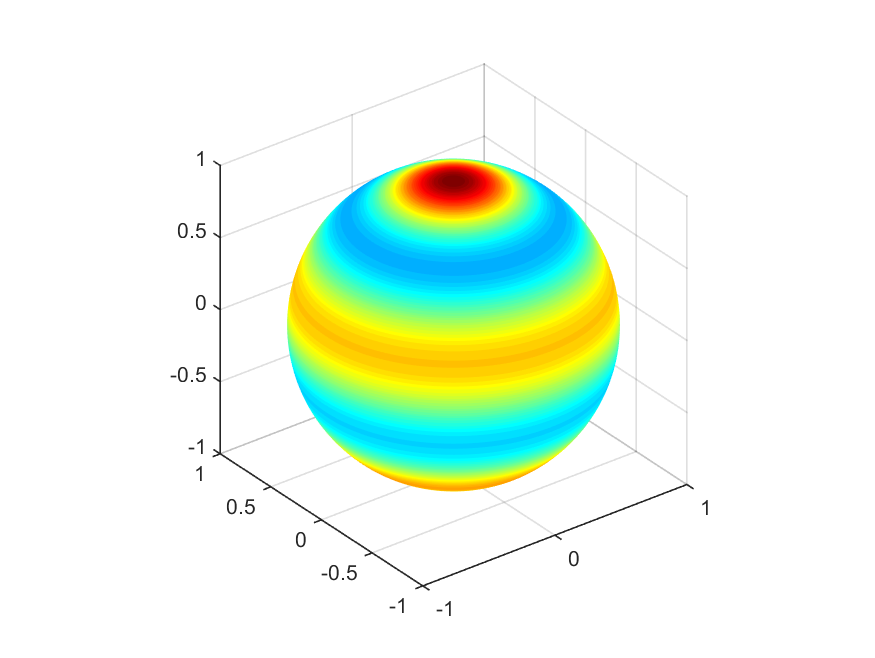
\includegraphics[width=1\textwidth]{chapters/images/ylm/a_5_0.pdf}
\caption{$Y^m_l$ mit $l=5$, $m=0$}
\label{skript:ylm l=5 m=0}
\end{minipage}
\hfill
\begin{minipage}[hbt]{0.4\textwidth}
\centering
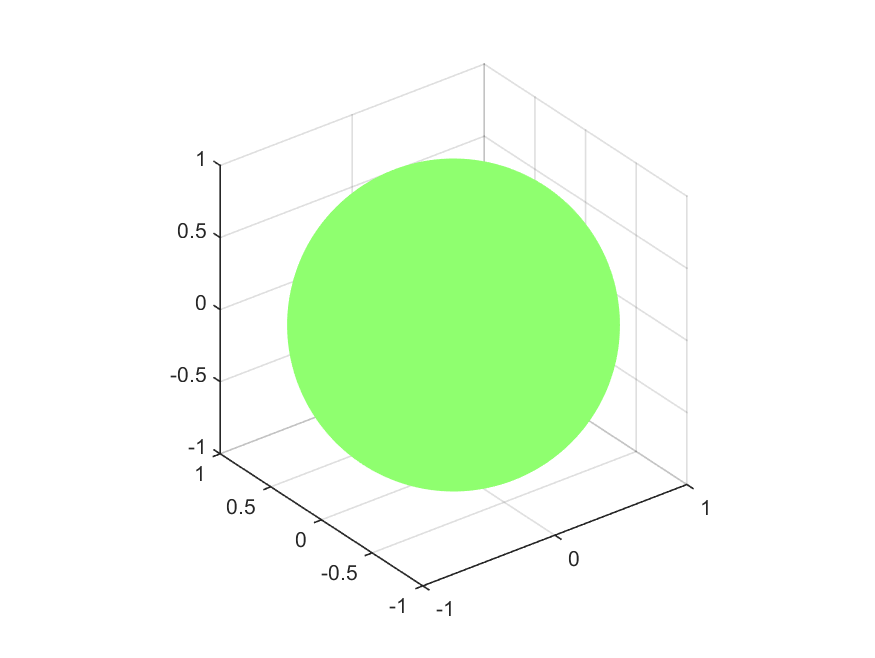
\includegraphics[width=1\textwidth]{chapters/images/ylm/b_5_0.pdf}
\caption{$Z_{lm}$ mit $l=5$, $m=0$}
\label{skript:zlm l=5 m=0}
\end{minipage}
\begin{minipage}[hbt]{0.4\textwidth}
\centering
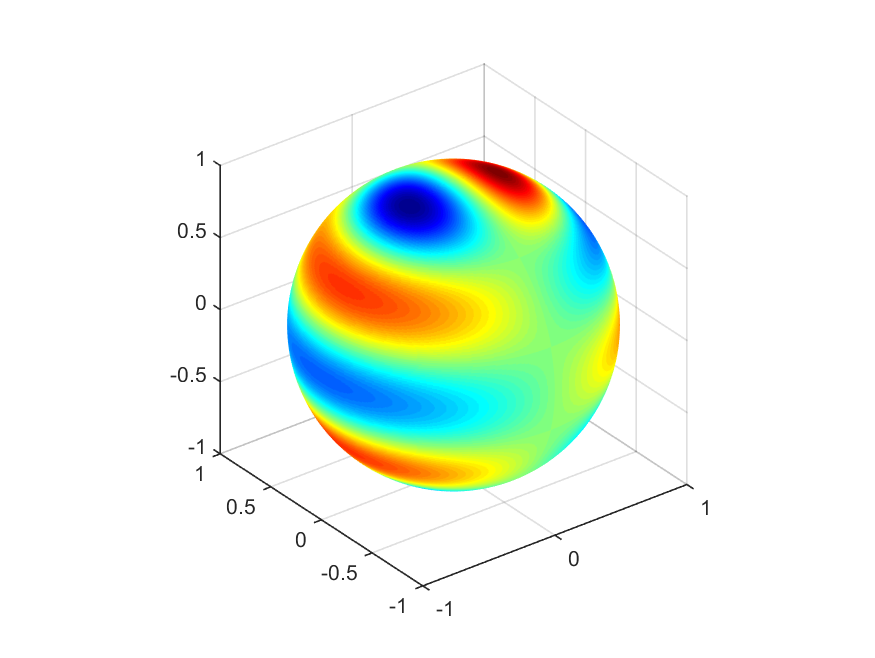
\includegraphics[width=1\textwidth]{chapters/images/ylm/a_5_1.pdf}
\caption{$Y^m_l$ mit $l=5$, $m=1$}
\label{skript:ylm l=5 m=1}
\end{minipage}
\hfill
\begin{minipage}[hbt]{0.4\textwidth}
\centering
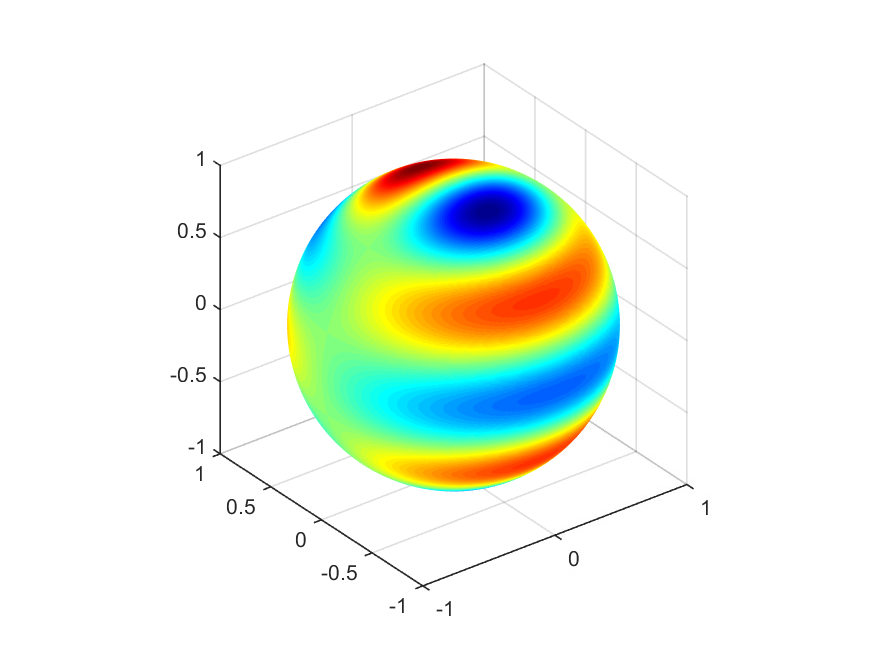
\includegraphics[width=1\textwidth]{chapters/images/ylm/b_5_1.pdf}
\caption{$Y^m_l$ mit $l=5$, $m=-1$}
\label{skript:zlm l=5 m=1}
\end{minipage}
\begin{minipage}[hbt]{0.4\textwidth}
\centering
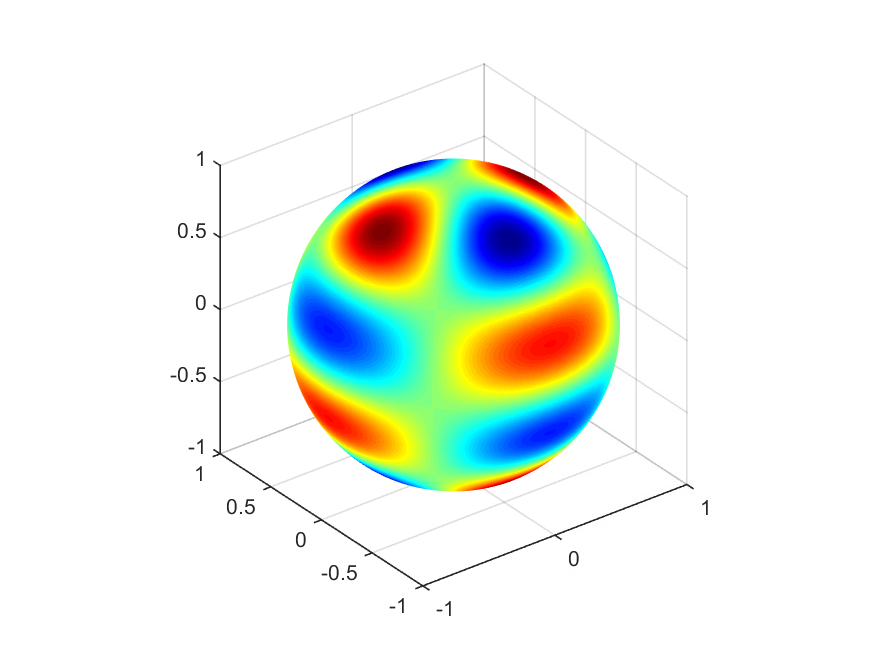
\includegraphics[width=1\textwidth]{chapters/images/ylm/a_5_2.pdf}
\caption{$Y^m_l$ mit $l=5$, $m=2$}
\label{skript:ylm l=5 m=2}
\end{minipage}
\hfill
\begin{minipage}[hbt]{0.4\textwidth}
\centering
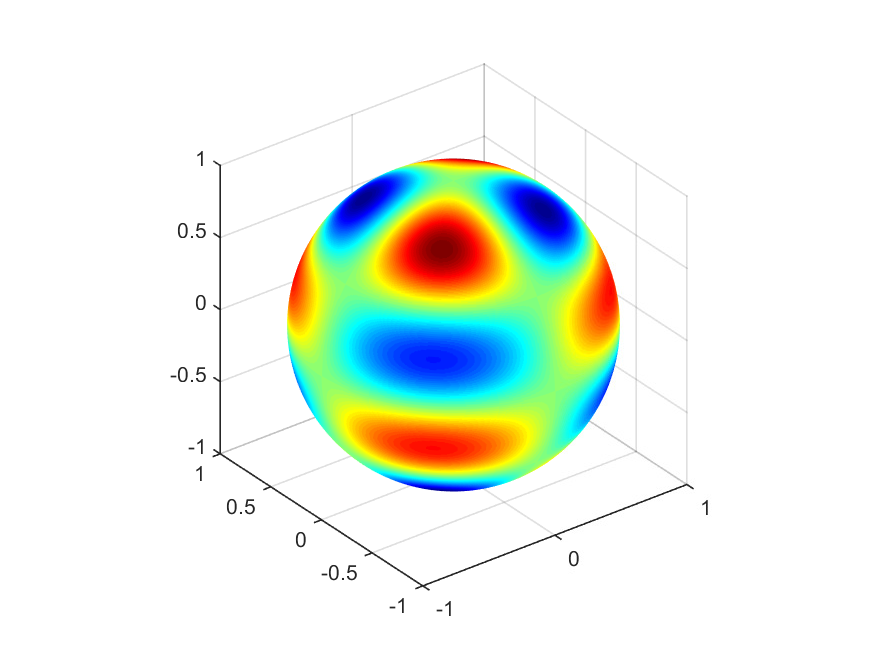
\includegraphics[width=1\textwidth]{chapters/images/ylm/b_5_2.pdf}
\caption{$Y^m_l$ mit $l=5$, $m=-2$}
\label{skript:zlm l=5 m=2}
\end{minipage}
\end{figure}

\begin{figure}
\begin{minipage}[hbt]{0.4\textwidth}
\centering
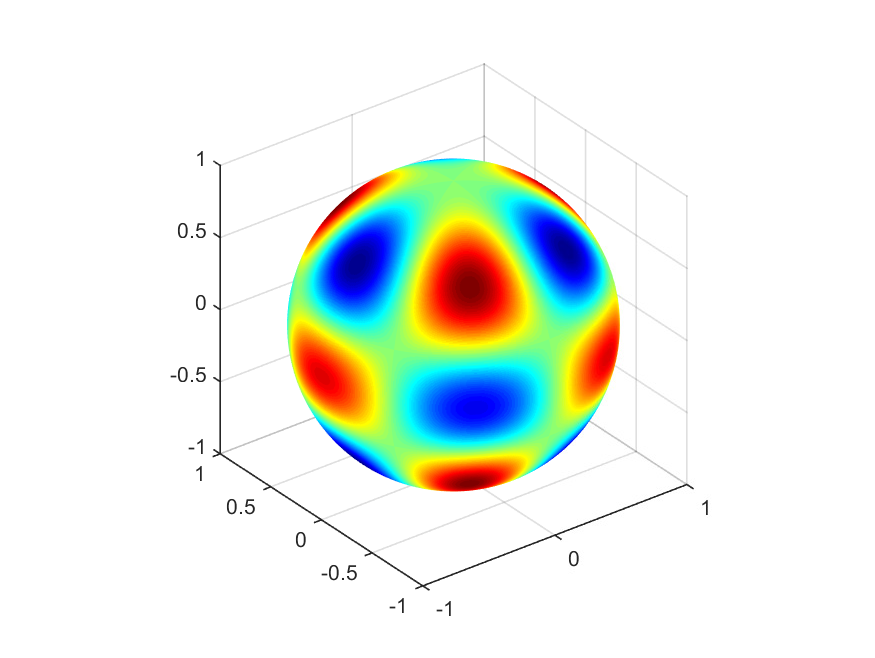
\includegraphics[width=1\textwidth]{chapters/images/ylm/a_5_3.pdf}
\caption{$Y^m_l$ mit $l=5$, $m=3$}
\label{skript:ylm l=5 m=3}
\end{minipage}
\hfill
\begin{minipage}[hbt]{0.4\textwidth}
\centering
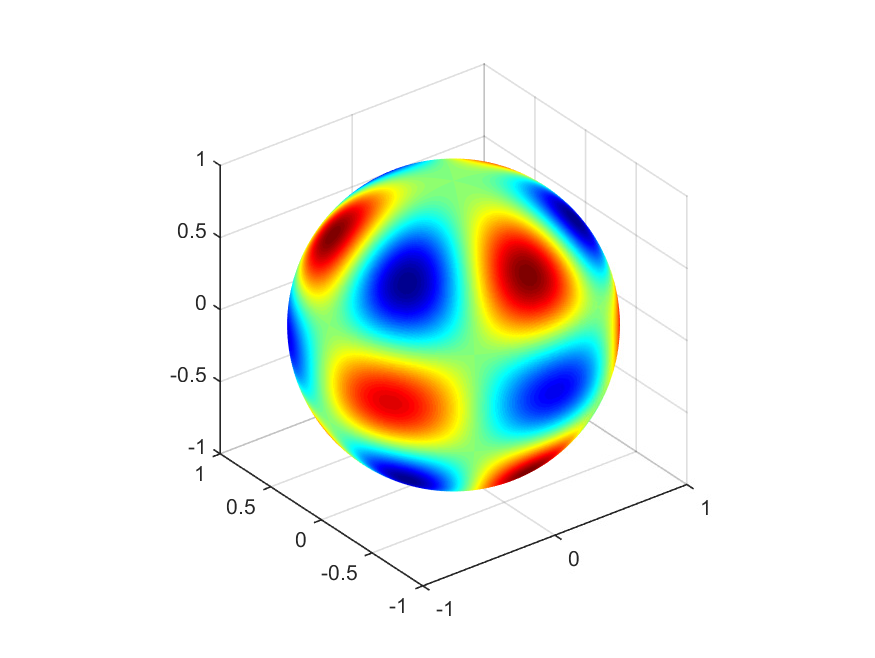
\includegraphics[width=1\textwidth]{chapters/images/ylm/b_5_3.pdf}
\caption{$Y^m_l$ mit $l=5$, $m=-3$}
\label{skript:zlm l=5 m=3}
\end{minipage}
\begin{minipage}[hbt]{0.4\textwidth}
\centering
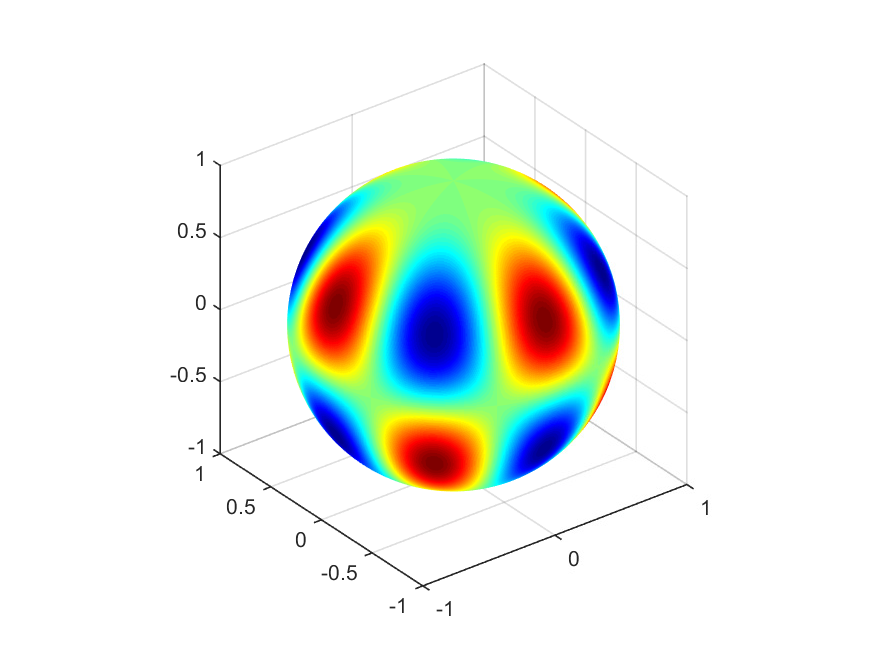
\includegraphics[width=1\textwidth]{chapters/images/ylm/a_5_4.pdf}
\caption{$Y^m_l$ mit $l=5$, $m=4$}
\label{skript:ylm l=5 m=4}
\end{minipage}
\hfill
\begin{minipage}[hbt]{0.4\textwidth}
\centering
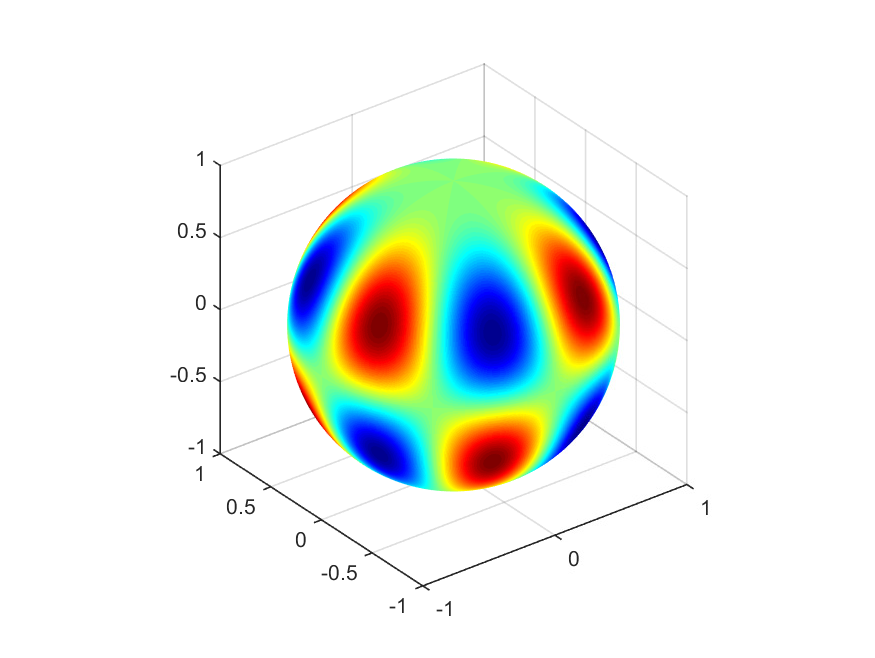
\includegraphics[width=1\textwidth]{chapters/images/ylm/b_5_4.pdf}
\caption{$Y^m_l$ mit $l=5$, $m=-4$}
\label{skript:zlm l=5 m=4}
\end{minipage}
\begin{minipage}[hbt]{0.4\textwidth}
\centering
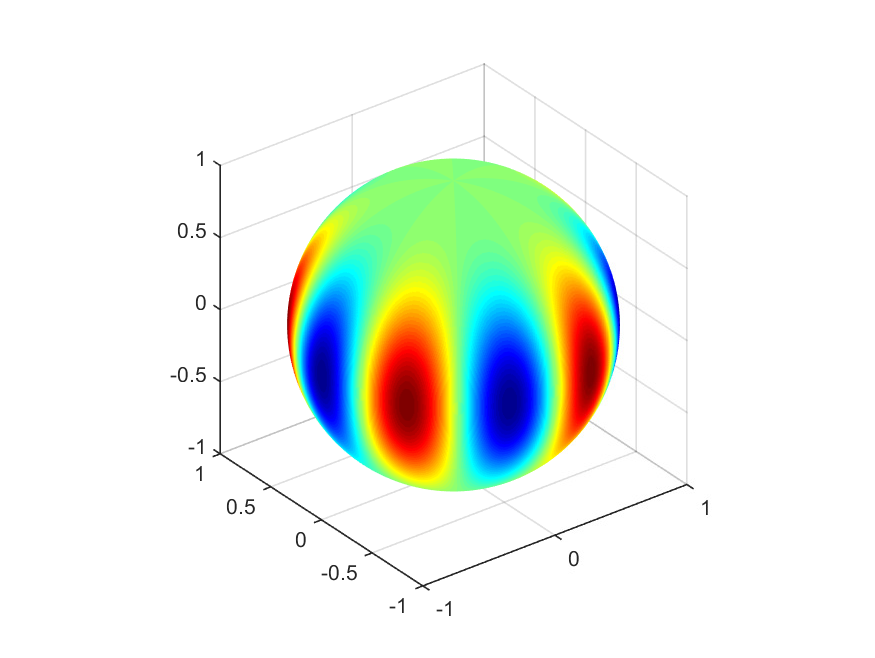
\includegraphics[width=1\textwidth]{chapters/images/ylm/a_5_5.pdf}
\caption{$Y^m_l$ mit $l=5$, $m=5$}
\label{skript:ylm l=5 m=5}
\end{minipage}
\hfill
\begin{minipage}[hbt]{0.4\textwidth}
\centering
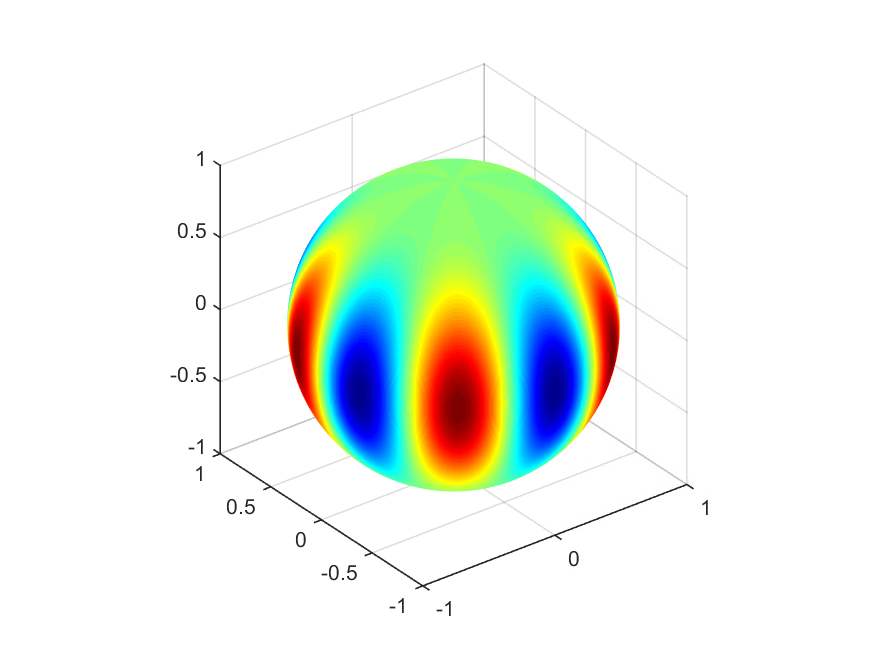
\includegraphics[width=1\textwidth]{chapters/images/ylm/b_5_5.pdf}
\caption{$Y^m_l$ mit $l=5$, $m=-5$}
\label{skript:zlm l=5 m=5}
\end{minipage}
\end{figure}

\subsection{Bedeutung einzelner Kugelfunktionskoeffizienten}
Einzelne Kugelfunktionskoeffizienten haben wie bei der klassischen
Fouriertheorie eine anschauliche Bedeutung.

Der Koeffizient $c_0^0$ ist
\[
c_0^0
=
\frac{N^0_0}{\sqrt{2\pi}}
\int_{-\pi}^\pi 
\int_0^\pi
f(\varphi,\vartheta)
\sin\vartheta
\,d\vartheta
\,d\varphi,
\]
also im Wesentlichen der Mittelwert der Funktione $f$ über die Kugeloberfläche.

Der Koeffizient $c^0_1$, also $l=1$ und $m=0$ ist der Koeffizient
zu der Funktion
\[
Y^0_1(\varphi,\vartheta)
=
\frac{N^0_1}{\sqrt{2\pi}} P_1(\cos\vartheta)
=
\frac{N^0_1}{\sqrt{2\pi}} \frac{1}{2}\frac{d}{dz}(z^2-1)
=
\frac{N^0_1}{\sqrt{2\pi}} z
=
\frac{N^0_1}{\sqrt{2\pi}} \cos\vartheta.
\]
Das Skalarprodukt $\langle f,Y^0_1\rangle$ ist also das
Integral
\[
\langle f,Y^0_1\rangle
=
\frac{N^0_1}{\sqrt{2\pi}}
\int_{-\pi}^\pi 
\int_0^\pi
f(\varphi,\vartheta)
\cos\vartheta
\sin\vartheta
\,d\vartheta
\,d\varphi
\]
Da $\cos\vartheta$ in der oberen Halbkugel postiv ist und in der 
unteren Halbkugel negativ, beschreibt der Koeffizient $c^0_1$ im
Wesentlichen den Unterschied zwischen den beiden Halbkugeln.















